\section{\DCME{}}\label{sec::dcme_dcme}

In this section, we present a \DCME{}~(DCME) approach which has two advantages
regarding learning and computational efficiency: (1) The model parameters
associated with \emph{all} items are updated at \emph{each} training instance;
and (2) The time complexity is independent of $N$.

\subsection{Primal-dual ME}

Different from existing approaches, DCME solves the ME problem in a primal-dual
fashion. Suppose that the dataset $\mathcal{D}$ has $M$ instances and $N$ items
where the $t$-th instance selects the $i_t$-th item. We start the derivation
from the primal ME formulation which maximizes the log-likelihood:

\begin{alignat}{-1}
  \sum\limits_{t=1}^M \log(\P_t(i_t; \THETA))=&
  \sum\limits_{t=1}^M \big(  f_t(i_t; \THETA)
  - \log \sum\limits_{j=1}^N \exp f_t(j; \THETA) \big) \nonumber\\
  =& \sum\limits_{t=1}^M \big(  f_t(i_t; \THETA) - A_t(\THETA) \big)
\label{eq::primal_ll}
\end{alignat}

where $A_t(\THETA)$ is referred to as the log-partition function and its
conjugate dual is revealed by the following
lemma~\cite{hiriart1993convex,wainwright2008graphical}:

\begin{lem}\label{lem::conj_dual}
  Assume $ \P(i; \vs) = \exp(s_i) / \sum\limits_{j=1}^N \exp(s_j)$
  and $A(\vs) = \log \sum\limits_{j = 1}^N \exp(s_j)$,
  the conjugate duality between the log-partition function and negative entropy
  states:

  \begin{align}
    A(\vs) &= \max\limits_{\vmu \in \Delta_N}
                    \{ \sum\limits_{j=1}^N \mu_j s_j -
                       \sum\limits_{j=1}^N \mu_j \log \mu_j \} \nonumber \\
           &= \max\limits_{\vmu \in \Delta_N}
                    \{ \E_{\vmu} [s_j] + \entropy(\vmu) \} \label{eq::conj_dual}
  \end{align}

  where the simplex set
  $\Delta_N = \{\mathbf{p} \in \mathbb{R}^{N}:
  p_j \ge 0, \sum\limits_{j=1}^N p_j = 1\}$

  and the maximizer is attained at:

  \begin{align}
    \mu_j^* = \P(j; \vs), \quad 1 \le j \le N \label{eq::conj_dual_sol}
  \end{align}

\end{lem}

\begin{proof}
  We use the following equivalence:
  \begin{align*}
    \E_{\vmu}[s_j] + \entropy(\vmu)
      &= -\sum\limits_{j=1}^N \mu_j \log \frac{\mu_j }{ \P(j; \vs) } +
          \log\sum\limits_{j=1}^N \exp(s_j) \nonumber \\
      &= -D_{KL}(\vmu || \P) + A(\vs)
  \end{align*}
where $D_{KL}(\vmu || \P)$ is the Kullback-Leibler (KL) divergence and note
$D_{KL}(\vmu || P) \ge 0$ and  $D_{KL}(P || P) = 0$. It follows that
$\vmu^* = \argmin\limits_{\vmu \in \Delta_N} D_{KL}(\vmu || P) = P$.
\end{proof}

In view of \Cref{lem::conj_dual}, we arrive at the primal-dual form of ME:

\begin{equation}
  \max\limits_\THETA
  \min\limits_{\substack{\vmu_t \in \Delta_N \\ 1 \le t \le M}}
  \sum\limits_{t=1}^M \big( f_t(i_t; \THETA) - \E_{\vmu_t}[f_t(j;\THETA)] -
  \entropy(\vmu_t) \big) \label{eq::me_primal_dual}
\end{equation}

where $\vmu_t$ is the \emph{dual distribution} for instance $t$.

\subsection{Dual Distribution Clustering}

\Cref{lem::conj_dual} implies that $\vmu_t^*$ is determined by $f_t(j;\THETA)$.
In less mathematical terms, similar instances choose similar items (in
probabilities). As real-world data instances generally possess a clustering
structure instead of being randomly distributed, it is expected that dual
distributions also form clusters. For the text classification example of venue
prediction, if papers are grouped by topics, those in the same group should have
similar chance of getting published at a particular venue; For learning word
embedding, we anticipate contexts of similar semantics yield target word
distributions that can be clustered together.

It is worth exploring the cluster structure of dual distributions to reduce
complexity. DCME rests on the idea of ``approximation by clustering'': By
clustering the dual distributions into $K$ groups, each $\vmu_t$ is assigned to
a cluster $c_t \in \{1, \dots K\}$, and is then approximated by the
corresponding \emph{cluster center} $\valpha_{c_t}\in\Delta_N$ which best
represents the group. The optimization problem of DCME can thus be formulated
as:

\begin{alignat}{-1}
  &\textrm{DCME:} && \qquad
\max\limits_\THETA
\min\limits_{\substack{\valpha_k \in \Delta_N \\ 1 \le k \le K}}
\min\limits_{\substack{1 \le c_t \le K \\ 1 \le t \le M}}
\sum\limits_{t=1}^M Q_t(\valpha_{c_t}; \THETA) \label{eq::dcme} \\
  &\textrm{where~~} &&
Q_t(\valpha_{c_t}; \THETA) =
  f_t(i_t;\THETA) -
  \E_{\valpha_{c_t}}[f_t(j;\THETA)] -
  \entropy(\valpha_{c_t})\big) \nonumber
\end{alignat}

\subsection{Online-Offline Optimization}

We employ Gauss-Seidel coordinate descent to solve \Cref{eq::dcme}.  Three
blocks of variables, namely, the model parameters $\THETA$, the cluster centers
$\{\valpha_k\}$, and the instances' cluster assignments $\{c_t\}$, are
successively updated while keeping others constant. In particular, we devise a
hybrid online-offline algorithm which breaks the computational bottleneck and
leads to a time complexity that only scales as $\oo(DK)$, as opposed to
$\oo(DN)$ in conventional ME algorithms.

\subsubsection{Updating cluster assignments~(Online)}

DCME approximates $\vmu_t$ by $\valpha_{c_t}$, and the cluster assignment $c_t$
is solved by:

\begin{equation}
  \argmin\limits_{1 \le k \le K} - \E_{\valpha_{k}}[f_t(j;\THETA)]
        - \entropy(\valpha_{k}) \label{eq::clu_mem}
\end{equation}

However, a na\"{i}ve computation would cost $\oo(DN + KN)$ time. It takes
$\oo(D)$ to evaluate $f_t(j;\THETA)$ for every item $1 \le j \le N$\footnote{In
  word embedding, one can compute the scoring function in $\oo(D)$ time. Note
  that the \emph{asymptotic} complexity of computing $\vhb_t$ in \emph{every}
sliding windows is $\oo(D)$ (independent of window size) with the sum $\sum_{-c
\le p \le c} \vh_{w_{t,p}}$ maintained by adding the new word and subtracting
the past word.}; For each cluster, another $\oo(N)$ is required to calculate
$\E_{\valpha_{k}}[f_t(j;\THETA)]$ and $\entropy(\valpha_k)$ by enumeration.

Fortunately, when the scoring function is linear in the feature/context vector,
the cost can be reduced to $\oo(DK)$ per instance. To see this, from
\eqref{eq::scr_classification} and \eqref{eq::scr_embedding} we have:

\begin{alignat}{-1}
  &\cc &
  \E_{\valpha_{k}}[f_t(j; \vW)] &= (\vW \valpha_{k})^T \vx_t
  \label{eq::exp_classification}\\
  &\ee &
  \E_{\valpha_{k}}[f_t(j; \vV,\vH)] &= (\vV \valpha_{k})^T \vhb_t
  \label{eq::exp_embedding}
\end{alignat}

The trick we apply here \emph{trades memory for time}: By storing $\vW
\valpha_{k}$, $\vV \valpha_{k}$ and $\entropy(\valpha_k)$ for $K$ clusters in
the offline update, it is merely a $D$-dimensional dot product to calculate
\Cref{eq::exp_classification} and \Cref{eq::exp_embedding}, and therefore the
cost to online update $c_t$ by \Cref{eq::clu_mem} is $\oo(DK)$.

\subsubsection{Updating cluster centers~(Offline)}

We update the cluster center $\valpha_k$ as well as the cached $\vW
\valpha_{k}$, $\vV \valpha_{k}$ and $\entropy(\valpha_k)$ only in the offline
computation. Let $\ii_k$ denote the index set of instances in the $k$-th
cluster, $\valpha_k$ satisfies:

\begin{align}
   \argmin\limits_{\valpha \in \Delta_N}
   -\E_{\valpha}\Bigg[\frac{1}{|\ii_k|}
                      \sum\limits_{t \in \ii_k}f_t(j; \THETA)\Bigg]
   -\entropy(\valpha) \label{eq::up_clu_center_opt}
\end{align}

Invoking \Cref{lem::conj_dual} again, \Cref{eq::up_clu_center_opt} has the
following closed-form solution:

\begin{align}
  \alpha_{k, j} = \frac{1}{Z} \exp\big(
      \frac{1}{| \ii_k |}
      \sum\limits_{t \in \ii_k} f_t(j;\THETA) \big)
  \label{eq::up_clu_center}
\end{align}

where a normalization term $Z$ is applied to keep $\sum\limits_{j=1}^N
\alpha_{k,j} = 1$. By the linearity of $f_t(j;\THETA)$, we express
\Cref{eq::up_clu_center} as:

\begin{alignat}{-1}
  &\cc & \quad
  \alpha_{k, j} = \frac{1}{Z} \exp\Big( \vw_j^T
  \frac{1}{| \ii_k |} \sum\limits_{t \in \ii_k} \vx_t\Big)
  \label{eq::up_clu_center_classification}\\
  &\ee &
  \alpha_{k, j} = \frac{1}{Z} \exp\Big( \vv_j^T
  \frac{1}{| \ii_k |} \sum\limits_{t \in \ii_k} \vhb_t\Big)
  \label{eq::up_clu_center_embedding}
\end{alignat}

which computes $\valpha_k$ with $\oo(D |\ii_k|  + D N)$ cost. In addition, it
takes $\oo(DN)$ and $\oo(N)$ to update $\vW \valpha_{k}$, $\vV \valpha_{k}$ and
$\entropy(\valpha_k)$, respectively. By choosing the interval between
consecutive offline updates such that $|\ii_k| = \beta N$ for a constant $\beta$
(1 for example), we obtain an average time complexity of $\oo(D)$ per instance.

\subsubsection{Updating model parameters~(Online/Offline)}

To optimize $\THETA$ with subgradient descent:

\begin{alignat}{-1}
  &\cc &
  \frac{\partial Q_t}{\partial \vw_j} &=
    \underbrace{\mathds{1}[i_t = j]\, \vx_t}_{(a)} +
    \underbrace{(-\alpha_{c_t, j} \vx_t)}_{(b)}
    \label{eq::mdl_upd_classification}\\
  &\ee &
  \frac{\partial Q_t}{\partial \vv_j} &=
    \overbrace{\mathds{1}[i_t = j]\, \vhb_t} +
    \overbrace{(-\alpha_{c_t, j} \vhb_t)}
    \label{eq::mdl_upd_embedding_v}\\
  &&
  \frac{\partial Q_t}{\partial \vh_{w_p^{(t)}}} &=
    \frac{1}{2c} (\vv_{i_t} - \vV \valpha_{c_t})
    \label{eq::mdl_upd_embedding_h}\\
  &&
  \textrm{for all}\; &-c \le p \le c,\; p \ne 0 \nonumber
\end{alignat}

where $\mathds{1}[i_t = j]$ is the indicator function which evaluates to 1 when
$i_t = j$ and 0 otherwise. In the following, we devise a hybrid
\emph{online-offline algorithm} which has an average expense of $\oo(D)$ time
per instance.

First, Term (a) in \Cref{eq::mdl_upd_classification} and
\Cref{eq::mdl_upd_embedding_v} only changes the model parameters associated with
the correct item $i_t$, namely $\vw_{i_t}$ and $\vv_{i_t}$, and can be updated
online in $\oo(D)$ time. Similarly, for word embedding
\Cref{eq::mdl_upd_embedding_h}, $\partial Q_t / \partial \vH$ can also be
updated online with $\oo(D)$ cost by keeping track of the sum of $\partial Q_t /
\partial \vh_{w}$ for all overlapping instances using a sliding window
technique.

Second, Term (b) in \Cref{eq::mdl_upd_classification} and
\Cref{eq::mdl_upd_embedding_v} changes the model parameters of all $N$ items.
We make two crucial observations here: (1) Term (b) of different items share the
\emph{same} direction $-\vx_t$ (or $-\vhb_t$); and (2) The scale vector
$\valpha_{c_t}$ \emph{only} depends on the cluster assignment $c_t$, but not the
individual instance $t$. Thus it is logical to perform offline update of Term
(b). The computation is postponed until $|\ii_{c_t}|$ is large enough, and then
Term (b) is calculated for all items $1 \le j \le N$ and instances $t \in
\ii_{c_t}$. Such ``lazy'' computation yields a total cost of $\oo(D |\ii_{c_t}|
+ D N)$, and we achieve an average $\oo(D)$ expense per instance if we wait
until $|\ii_{c_t}| \ge \beta N$.

\subsubsection{Tuning online/offline computation}

The overall complexity per instance is $\oo(DK)$ time, which is appealing as it
does not hinge on $N$.  Nevertheless, an inherent limitation in learning is the
delay of computing Term (b) until $|\ii_k| \ge \beta N$ in
\Cref{eq::mdl_upd_classification} and \Cref{eq::mdl_upd_embedding_v} ,
especially for items with large values $\alpha_{k, j}$. A heuristic improvement
we find effective in practice tunes the computation between online and offline
updates. By sorting items (using a heap) with decreasing $\alpha_{k,j}$, Term
(b) of the top $Q$ items are updated online while the others are updated
offline. The resulting average cost per instance becomes $\oo(D K + D Q + \log
Q)$. Computational efficiency is preferred with a small $Q$ while the priority
shifts to learning efficiency with a large $Q$.

\section{DCME Algorithm}\label{sec::dcme_algo}

\subsection{Overall Procedures}

We summarize the learning procedure of DCME in \Cref{alg::dcme}. DCME assigns
each training instance $t$ to a dual cluster $c_t$ and performs the online model
update. Once the size of a dual cluster reaches $\beta N$, an offline model
update as well as the update of the dual cluster center are applied.  Although
the algorithm has a similar complexity as the sampling-based approaches such as
noise contrastive estimation~(NCE) and negative sampling~(NS), DCME allows the
\emph{entire} model to learn from \emph{every} training instance. In other
words, the model parameters associated with all items get updated when a new
training instance arrives, which yields superior performance over existing
methods, as will be shown in the experimental study.

\begin{algorithm}[h]
\caption{DCME algorithm}\label{alg::dcme}
  % \SetAlgoNoLine
  \KwIn{$M$ instances, a constant $\beta$, cluster number $K$, and top item
        number $Q$}
	\KwOut{Model $\mathbf{\THETA}$}
  Initialize $K$ clusters $\{\valpha_k\}$ \;
	\While{$\THETA$ is not optimal}{
    \begin{itemize}
      \item[--] Select an index $t$ from $\{1, \dots, M\}$
      \item[--] Find the cluster assignment $c_t$ by \eqref{eq::clu_mem}
      \item[--] Perform online update of Term (a) (and Term (b) of the \\
                 top $Q$ items) in \eqref{eq::mdl_upd_classification} (or
                \eqref{eq::mdl_upd_embedding_v}). For embedding, also \\
                update $H$ by \eqref{eq::mdl_upd_embedding_h}.
      \item[--] Add $t$ to $\ii_{c_t}$; \\
                if $|\ii_{c_t}| \ge \beta N$
        \begin{itemize}
          \item[--] Perform offline update of Term (b) in
                    \eqref{eq::mdl_upd_classification} (or
                    \eqref{eq::mdl_upd_embedding_v}).
          \item[--] Update cluster center $\alpha_{c_t}$ and empty
                    $\ii_{c_t}$
        \end{itemize}
    \end{itemize}
	}
\end{algorithm}

\subsection{Connection with K-means}

So far, readers might have already been aware of the resemblance between the
dual distribution clustering and the K-means algorithm. The following theorem
formally proves their connection:

\begin{thm}
  The dual distribution clustering in DCME is a generalized K-means
  algorithm using KL-divergence as the distance measurement in the simplex.
  Moreover, it converges as fast as K-means.
\end{thm}
\begin{proof}
  Using \Cref{lem::conj_dual}, the dual clustering satisfies:

  \begin{alignat}{-1}
    \min\limits_{\substack{\valpha_k\in \Delta_N ,  1 \le k \le K \\
                           1 \le c_t \le K , 1 \le t \le M}} \;
  \sum\limits_{t=1}^M D_{KL}(\valpha_{c_t} || P_t) \label{eq::k-means_clustering}
  \end{alignat}

  which minimizes the \emph{within-cluster KL-divergence} between
  $\valpha_{c_t}$ and $P_t$. It is the same minimization objective as K-means
  except that DCME measures the distance in the simplex space with
  KL-divergence\footnote{Technically, KL-divergence is not a true metric of
  distance.}. To illustrate this, notice that the dual clustering proceeds by
  alternating between the following two steps (See \Cref{fig::dual_cluster}):

\begin{itemize}
\item[--] Update $c_t = \argmin_{k} D_{KL}(\valpha_k || P_t)$, and $t$ is
  assigned to the cluster whose center is nearest to $P_t$ by KL-divergence.
\item[--] Update $\valpha_k = \argmin_{\valpha} \sum_{t \in \ii_k} D_{KL}(
  \valpha || P_t)$ where the cluster center is found as the point in the simplex
  with the least within-cluster distance.
\end{itemize}

General convergence results for the subgradient methods can be applied.
Specifically, the above two-step algorithm converges to the local minimum of the
problem \eqref{eq::k-means_clustering} as fast as the K-means
algorithm~\cite{bottou1995convergence},
\end{proof}

\begin{figure}[h!]
  \centering
  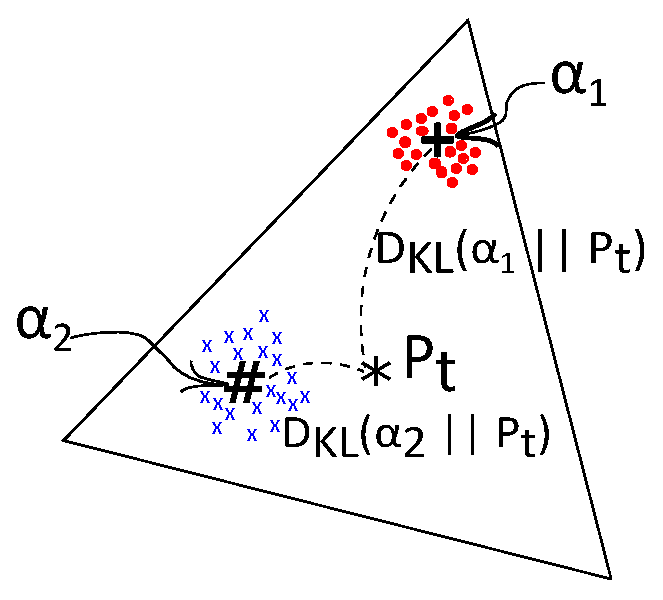
\includegraphics[width=0.4\linewidth]{dcme/dual_cluster_color.eps}
  \caption{Dual Clustering in the Simplex with KL-divergence}
  \label{fig::dual_cluster}
\end{figure}

\subsection{Connection with Dual ME}

The DCME is reminiscent of the dual ME, and we show the following results in the
classification setting:

\begin{thm} The dual form of DCME in classification is:
  \begin{align}
    \max\limits_{\substack{\valpha_k \in \Delta_N ,  1 \le k \le K \\
                           1 \le c_t \le K , 1 \le t \le M}}
                 &\qquad
    \sum\limits_{t=1}^M \entropy(\valpha_{c_t}) \label{eq::dual_dcme_op} \\
    \subjto \quad
    & \sum\limits_{t = 1}^M \mathds{1}[i_t = j]\; \vx_t =
    \sum\limits_{t = 1}^M \alpha_{c_t, j} \vx_t,~~ 1 \le j \le N \nonumber
  \end{align}
\end{thm}

The proof is omitted because it is very similar to the derivation of dual ME.
However, the dual form of DCME provides us with intuition of how DCME works: To
approximate $P_t$, the cluster center is restricted to reproduce the observed
statistics. Comparing it with the dual ME where $\vmu_t$ is in place of
$\valpha_{c_t}$, we see that the dual DCME has more restricted constraints. A
limiting case that DCME becomes identical to ME is when $K=M$, \ie{} each
instance is a singleton cluster with the only member being itself.
